\documentclass{article}
\usepackage[utf8]{inputenc}
\usepackage[T1]{fontenc}
\usepackage[table,xcdraw]{xcolor}
\usepackage{graphicx}
\begin{titlepage}

\begin{center}

  \LARGE \textsc{Politechnika Wrocławska}\\
  \vspace*{0.2cm}
  \Large \textsc{Wydział Informatyki i Telekomunikacji}\\
  \vspace*{0.4cm}
  \centering
\includegraphics[width=0.2\textwidth]{WITlogo.png}\\
  \vspace*{0.2cm}
  \vspace*{2cm}

  \centerline{\rule{\textwidth}{1.2pt}}
  \vspace{0.4cm}
  \Huge\textbf{Metody i Systemy Decyzyjne}
  \centerline{\rule{\textwidth}{1.2pt}}
  \vspace{1cm}
  \LARGE Sprawozdanie z laboratorium\\
  \vspace{3.5cm}
  \textsc{Autor}\\
  \vspace{0.2cm}
  \textbf{Jakub Roszkowski}\\
  \vspace{0.1cm}
  \Large nr albumu: \textbf{260282}\\
  \vspace{0.1cm}
  kierunek: \textbf{Informatyka Stosowana}

  \vspace*{\fill}
  \Large \textit{\today}

 \end{center}


\end{titlepage}


\title{Analiza czy po rozmiarze dłoni można określić parametry fizyczne osoby}
\date{\today}

\usepackage{float} 
\begin{document}

\maketitle

\tableofcontents
\newpage

\section{Wstęp}
\subsection{Wybór data setu oraz problemu do analizy}

Poszukując zbioru danych do analizy, zainteresował mnie ten dotyczący pomiarów dłoni oraz parametrów fizycznych osób. Celem analizy jest zbadanie czy
wielkość dłoni ma jakiś związek ze wzrostem i wagą

\subsection{Źródło data setu}

Data set analizowany w dalszej części raportu został pobrany ze strony:\\
\textbf{https://www.kaggle.com/code/seshadrikolluri/anthropometric-data-analysis-and-visualization/data?select=ANSUR+II+FEMALE+Public.csv}
\newpage


\section{Preprocessing danych}
\subsection{Wybór danych poddanych analizie}
Wybrany data set posiadał na wstępie 108 kolumn danych. Spośród nich wyłoniłem 6 które moim zdaniem mogły wpłynąć w pewnym stopniu na rozpatrywane wyniki. 
\begin{itemize}
    \item hand breadth - kolumna zawierające dane na temat szerokości dłoni w milimetrach.
    \item hand circumference - kolumna zawierające dane na temat obwodu dłoni w milimetrach.
    \item hand length - kolumna zawierające dane na temat długości dłoni w milimetrach.
    \item Gender - kolumna zawierająca dane na temat płci
    \item Weight - kolumna zawierająca dane na temat wagi w kilogramach
    \item Height - kolumna zawierająca dane na temat wzrostu w centymetrach
\end{itemize}

\subsection{Przetworzenie danych}
Zmieniłem wartości wagi z funtów na kilogramy oraz wartości wysokości z cali na centymetry. Musiałem również połączyć dwie bazy danych w jedną ponieważ były one rozdzielne na mężczyzn i kobiety. Postanowiłem również zmienić wartości płci z Female na 0 oraz z Male na 1

Nieznacznie zmieniłem również nazwy kolumn na takie które wydają mi się bardziej przejrzyste.



\begin{subsection} {Rozkłady danych}

\begin{figure}[H]
    \centering
    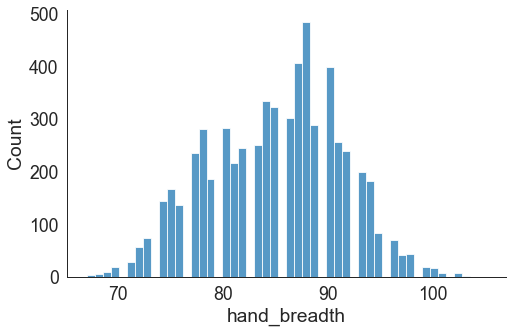
\includegraphics[width=8cm]{hand breadth.png}
    \caption{Rozkład danych - hand breadth}
    \label{fig:my_img}
\end{figure}


\begin{figure}[H]
    \centering
    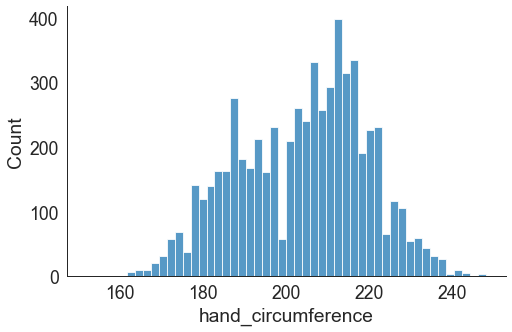
\includegraphics[width=8cm]{hand_circumference.png}
    \caption{Rozkład danych - hand circumference}
    \label{fig:my_img}
\end{figure}

\begin{figure}[H]
    \centering
    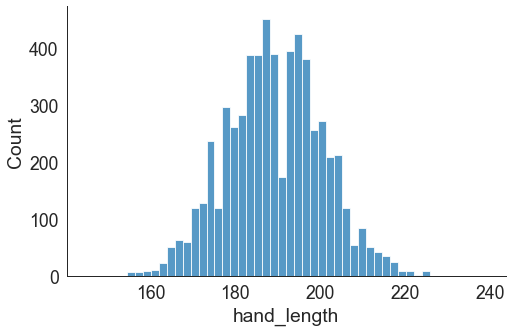
\includegraphics[width=8cm]{hand_length.png}
    \caption{Rozkład danych - hand length}
    \label{fig:my_img}
\end{figure}

\begin{figure}[H]
    \centering
    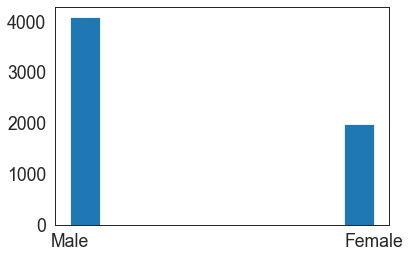
\includegraphics[width=8cm]{plec.png}
    \caption{Rozkład danych - Gender}
    \label{fig:my_img}
\end{figure}

\begin{figure}[H]
    \centering
    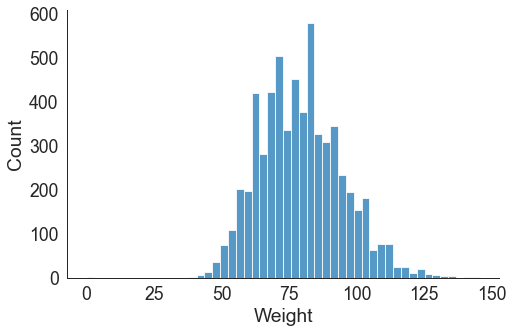
\includegraphics[width=8cm]{Weight.png}
    \caption{Rozkład danych - Weight}
    \label{fig:my_img}
\end{figure}

\begin{figure}[H]
    \centering
    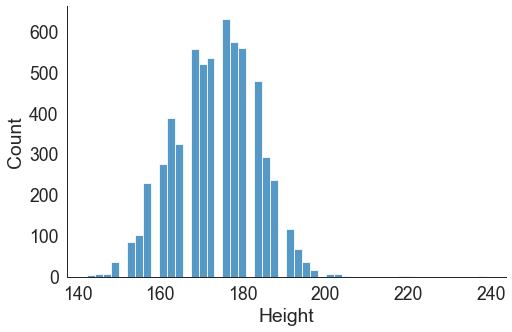
\includegraphics[width=8cm]{Height.png}
    \caption{Rozkład danych - Height}
    \label{fig:my_img}
\end{figure}

\begin{figure}[H]
    \centering
    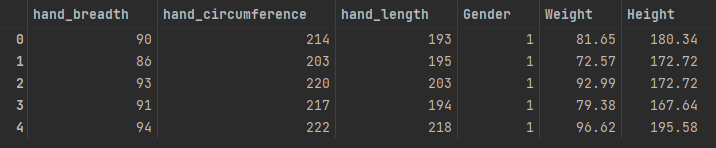
\includegraphics[width=12cm]{dane.png}
    \caption{Rozkład danych - przykladowe wartości danych}
    \label{fig:my_img}
\end{figure}

\begin{figure}[H]
    \centering
    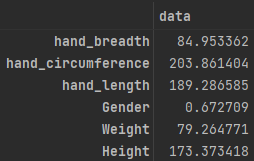
\includegraphics[width=8cm]{srednie_dane.png}
    \caption{Rozkład danych - średnie wartości danych}
    \label{fig:my_img}
\end{figure}
\end{subsection}


\newpage
\section{Rozwiązanie probelmu}
\subsection{Opis problemu}
Celem analizy jest próba:

\subsubsection{Dopasowanie rozkładu do wartości długości dłoni}
\subsubsection{Dopasowanie modeli regresji: liniowej, GLM i SVR modelującego wzrost człowieka na podstawie jednego z parametrów dłoni}
\subsubsection{Dopasowanie modeli regresji: liniowej, GLM i SVR modelującego wagę człowieka na podstawie jednego z parametrów dłoni}
\subsubsection{Klasyfikacja płci na podstawie pomiarów dłoni}

\subsection{Podział danych testowych}
Wszystkie dane użyte do wyznaczenia regresji jak i klasyfikatora w kolejnych etapach, dziele na dane trenujące jaki i testowe w proporcji 75:25 z ustawionym ziarnem losowości na 143 aby dane były losowane zawsze w ten sam sposób. Analizować będę modele stworzone na podstawie estymatorów dostępnych w sckit-learn.




\newpage
\section{Wykonywane eksperymenty z modelami / rozkładami}
\subsection{Dopasowanie rozkładu do wartości długości dłoni}
Na początku za pomocą modułu fitter opartym na module SciPy określę wartości błędu kwadratowego dla kilku popularnych rozkładów tj. Normalnego, Gamma, Chi2 oraz Cauchy’ego

Jakość każdego dopasowania określamy błędem średnio-kwadratowym
\begin{center}
\begin{tabular}{ |c|c| } 
 \hline
 Rozkład & Błąd \\ 
 \hline
 \hline
 Normalny & 0.003132 \\ 
 \hline
 Gamma & 0.003271 \\
 \hline
 Chi2 & 0.003427 \\
 \hline
 Cauchy’ego & 0.004453 \\ 
 \hline
\end{tabular}
\end{center}
Najlepszym rozkładem okazał się rozkład normalny
\begin{figure}[H]
    \centering
    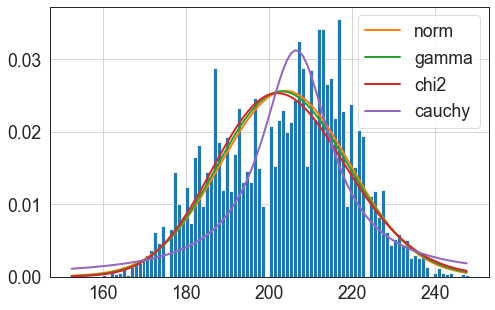
\includegraphics[width=8cm]{rozklady.png}
    \caption{Próba dopasowania kilku popularnych rozkładów do danych długości dłoni}
    \label{fig:my_img}
\end{figure}





\newpage
\subsection{Dopasowanie modeli regresji: liniowej, GLM i SVR modelującego wzrost człowieka na podstawie jednego z parametrów dłoni}
Po analizie współczynnika korelacji możemy wywnioskować że atrybutem najlepiej odwzorowującym wartość wzrostu jest pomiar długości ręki. Dlatego też wybieramy ją na daną naszego modelu.
\begin{figure}[H]
    \centering
    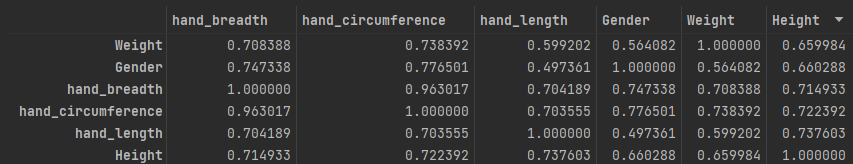
\includegraphics[width=12cm]{Height_corr.png}
    \caption{Tabela korelacji}
    \label{fig:my_img}
\end{figure}
Za pomocą danych testujących zostały stworzone 3 modele: regresji liniowej, GLM jak i SVR. Parametry modeli, błąd średnio-kwadratowy (Mean Square Error (MSE)) jak i uśredniony błąd bezwględny (Mean Absolute Error (MAE)) tych modeli został ukazany w Tabeli
\begin{center}
\begin{tabular}{ |c|c|c|c| } 
 \hline
 Model & Parametry & MSE & MAE  \\ 
 \hline
 \hline
 Liniowy & [0.63239], 53.74442 & 44.8 & 5.09 \\ 
 \hline
 GLM & [ 0.      2.0747 -0.0038], -82.48953 & 44.3 & 5.07 \\
 \hline
 SVR  & ——– & 44.6 & 5.08   \\
 \hline
\end{tabular}
\end{center}
\begin{figure}[H]
    \centering
    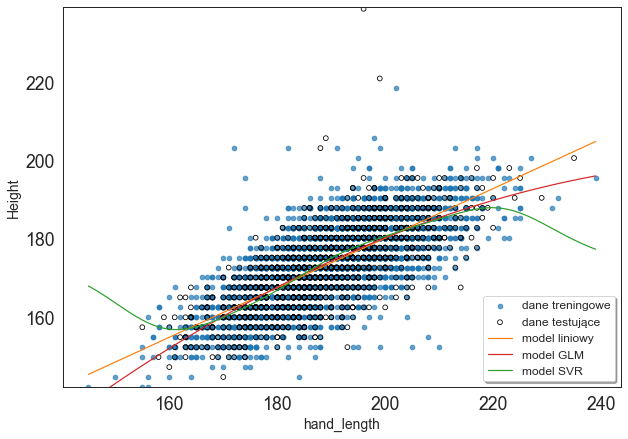
\includegraphics[width=10cm]{modelregresjiwysokosc.png}
    \caption{Modele regresji próbujące opisać wzrost człowieka względem długości dłoni}
    \label{fig:my_img}
\end{figure}


\newpage
Dodatkowo warto sprawdzić czy wartość błędu zmieni się gdy uwzględnimy dane mężczyzn i kobiet osobno. 
\begin{center}
tabela kobiet
\end{center}
\begin{center}
\begin{tabular}{ |c|c|c|c| } 
 \hline
 Model & Parametry & MSE & MAE  \\ 
 \hline
 \hline
 Liniowy & [0.42635], 86.89839 & 31.7 & 4.37 \\ 
 \hline
 GLM & [ 0.      1.4223 -0.0027], -3.7936, -82.48953 & 31.6 & 4.36 \\
 \hline
 SVR  & ——– & 32.5 & 4.4   \\
 \hline
\end{tabular}
\end{center}

\begin{figure}[H]
    \centering
    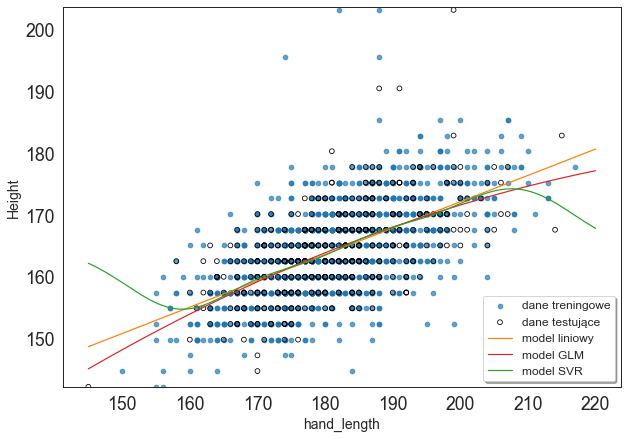
\includegraphics[width=10cm]{modelregresjiwysokosc_women.png}
    \caption{Modele regresji próbujące opisać wzrost kobiety względem długości dłoni}
    \label{fig:my_img}
\end{figure}

\newpage
\begin{center}
tabela mężczyzn
\end{center}
\begin{center}
\begin{tabular}{ |c|c|c|c| } 
 \hline
 Model & Parametry & MSE & MAE  \\ 
 \hline
 \hline
 Liniowy & [0.48744], 83.68982 & 35.9 & 4.51 \\ 
 \hline
 GLM & [ 0.      1.2108 -0.0019], 13.53194 & 35.8 & 4.5 \\
 \hline
 SVR  & ——– & 36.0 & 4.52   \\
 \hline
\end{tabular}
\end{center}

\begin{figure}[H]
    \centering
    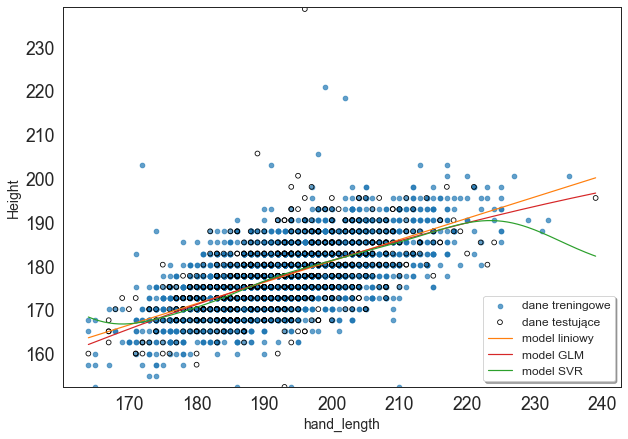
\includegraphics[width=10cm]{modelregresjiwysokosc_men.png}
    \caption{Modele regresji próbujące opisać wzrost mężczyzny względem długości dłoni}
    \label{fig:my_img}
\end{figure}
Z doświadczenia wynika że można określić wrost człowieka na podstawie długości ręki, już dla ogólnej bazy wartości są dosyć dokładne, jenak przy odróżnieniu płci wartości są jeszcze dokładniejsze.






\newpage
\subsection{Dopasowanie modeli regresji: liniowej, GLM i SVR modelującego wagę człowieka na podstawie jednego z parametrów dłoni}
Po analizie współczynnika korelacji możemy wywnioskować że atrybutem najlepiej odwzorowującym wartość wzrostu jest pomiar obwodu ręki. Dlatego też wybieramy ją na daną naszego modelu.
\begin{figure}[H]
    \centering
    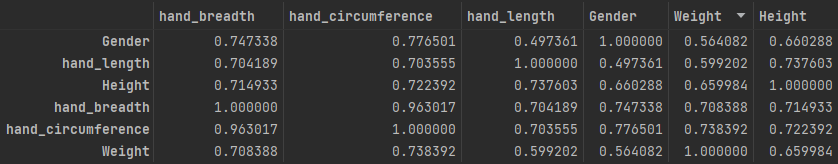
\includegraphics[width=12cm]{Weight_corr.png}
    \caption{Tabela korelacji}
    \label{fig:my_img}
\end{figure}
Za pomocą danych testujących zostały stworzone 3 modele: regresji liniowej, GLM jak i SVR. Parametry modeli, błąd średnio-kwadratowy (Mean Square Error (MSE)) jak i uśredniony błąd bezwględny (Mean Absolute Error (MAE)) tych modeli został ukazany w Tabeli
\begin{center}
\begin{tabular}{ |c|c|c|c| } 
 \hline
 Model & Parametry & MSE & MAE  \\ 
 \hline
 \hline
 Liniowy & [0.73261], -70.04801 & 1.04e+02 & 7.99 \\ 
 \hline
 GLM & [ 0.     -0.2449  0.0024], 28.19685, -82.48953 & 1.04e+02 & 7.98 \\
 \hline
 SVR  & ——– & 1.05e+02 & 7.98   \\
 \hline
\end{tabular}
\end{center}
\begin{figure}[H]
    \centering
    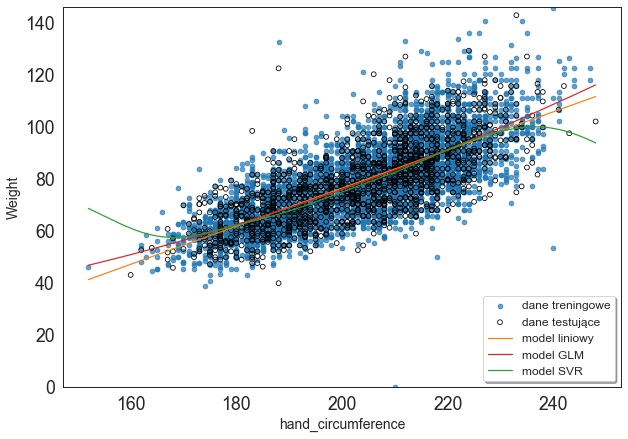
\includegraphics[width=10cm]{modelregresjiwaga.png}
    \caption{Modele regresji próbujące opisać wagę człowieka względem obwodu dłoni}
    \label{fig:my_img}
\end{figure}


\newpage
Dodatkowo warto sprawdzić czy wartość błędu zmieni się gdy uwzględnimy dane mężczyzn i kobiet osobno. 
\begin{center}
tabela kobiet
\end{center}
\begin{center}
\begin{tabular}{ |c|c|c|c| } 
 \hline
 Model & Parametry & MSE & MAE  \\ 
 \hline
 \hline
 Liniowy & [0.66795], -57.68512 & 73.3 & 6.82 \\ 
 \hline
 GLM & [ 0.     -0.1457  0.0022], 18.18156 & 73.6 & 6.82 \\
 \hline
 SVR  & ——– & 73.6 & 6.77   \\
 \hline
\end{tabular}
\end{center}

\begin{figure}[H]
    \centering
    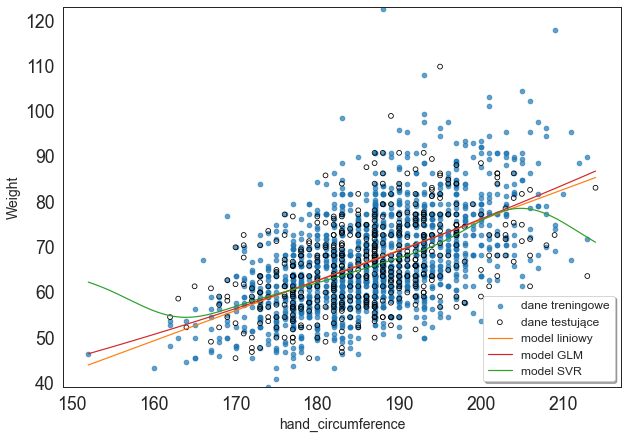
\includegraphics[width=10cm]{modelregresjiwaga_women.png}
    \caption{Modele regresji próbujące opisać wagę kobiety względem obwodu dłoni}
    \label{fig:my_img}
\end{figure}

\newpage
\begin{center}
tabela mężczyzn
\end{center}
\begin{center}
\begin{tabular}{ |c|c|c|c| } 
 \hline
 Model & Parametry & MSE & MAE  \\ 
 \hline
 \hline
 Liniowy & [0.79419], -83.30662 & 1.08e+02 & 8.23 \\ 
 \hline
 GLM & [0.     0.4009 0.0009], -41.56403 & 1.08e+02 & 8.23 \\
 \hline
 SVR  & ——– & 1.08e+02 & 8.19   \\
 \hline
\end{tabular}
\end{center}

\begin{figure}[H]
    \centering
    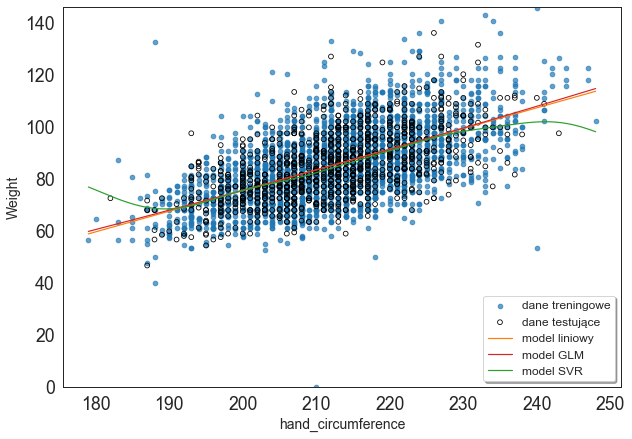
\includegraphics[width=10cm]{modelregresjiwaga_men.png}
    \caption{Modele regresji próbujące opisać wagę mężczyzny względem obwodu dłoni}
    \label{fig:my_img}
\end{figure}

Z doświadczenia wynika ciekawy wynik, co prawda błędy zarówno u mężczyzn jak i kobiet są dosyć duże, jednak u kobiet błedy są znacznie mniejsze niż u mężczyzn.




\subsection{Klasyfikacja płci na podstawie pomiarów dłoni}
Jak mogliśmy zauważyć dzięki znajomości płci jesteśmy wstanie lepiej określić pewne wartości fizyczne osób. Więc postaramy się ją wyznaczyć. Za pomocą danych opisujących wartości parametrów odcisku palca jak i płci uczestników badania tworzymy klasyfikator. Naszym klasyfikatorem będzie KNN (K-Nearest Neighbours) z biblioteki scikit-learn, określający klasę/wartość(u nas płeć) na podstawie odległości od K -sąsiadów. Nasze dane na tych samych zasadach dzielimy na testowe i trenujące co w poprzednich eksperymentach. Natomiast K ustawiamy równe 7.
Dokładność rozwiązania tego klasyfikatora wynosi 94\% czyli z całkiem dużą dokładnością możemy określić płeć osoby na podstawie jej odcisku palca.





\section{Wnioski}

Wnioskując z wykonanych eksperymentów można dowiedzieć się, że można przewidzieć wzrost jak i wagę
człowieka za pomocą dłoni poprzez modele regresji. Całkiem ważnym aspektem jest zaznaczenie tego że
dokładniej można określić wzrost, gdy wiemy jaka jest płeć poszukiwanej osoby. Natomiast gdy nie mamy takiej informacji, możemy ją łatwo uzyskać. Dostaniemy ją za pomocą klasyfikatora KNN (Eksperyment III-D) którego danymi są pomiary dłoni. Jesteśmy w stanie z 94 \% poprawnością określić czy dana osoba jest kobietą czy mężczyzną tylko za pomocą kilku parametrów dotyczących ręki. Natomiast określenie wagi osoby nie jest aż tak właściwe za pomocą modeli regresji ponieważ jest obarczone dość dużym błędem.Zważając nawet na te błędy modeli. Wartości pomiarów ręki, mogą służyć do całkiem trafnego określeniu wzrostu oraz wagi. Jednak musimy się liczyć że nasz model jest obarczony pewnym błędem w przypadku wzrostu mniejszym a wagi większym.


\end{document}